%\documentclass[twoside]{scrartcl}
%%%%%%%%%%%%%%%%%%%%%%%%%%%%%%%%%%%%%%%%%%%%%%%%%%%%%%%%%%%%%%%%%%%%%%%
%% Optionen zum Layout des Buchs                                     
%\documentclass[a4paper]{scrbook}
%\documentclass[a4paper, fontsize=14pt]{scrbook}
%\usepackage{etex}
%\usepackage{morefloats}
%\usepackage[17pt]{extsizes}
%\usepackage{morefloats}
%\KOMAoptions{fontsize=14pt} 
%
%%
%%%%%%%%%%%%%%%%%%%%%%%%%%%%%%%%%%%%%%%%%%%%%%%%%%%%%%%%%%%%%%%%%%%%%%%
%\documentclass{scrartcl} 
\documentclass[a4paper,							% alle weiteren Papierformat einstellbar
%landscape,						% Querformat
%10pt,								% Schriftgröße (12pt, 11pt (Standard))
%12pt,
fontsize=14pt,
%BCOR1cm,							% Bindekorrektur, bspw. 1 cm
%DIVcalc,							% fährt die Satzspiegelberechnung neu aus
%											  s. scrguide 2.4
%oneside,							% einseitiges Layout
%twocolumn,						% zweispaltiger Satz
%openany,							% Kapitel kännen auch auf linken Seiten beginnen
%halfparskip*,				% Absatzformatierung s. scrguide 3.1
%headsepline,					% Trennline zum Seitenkopf	
%footsepline,					% Trennline zum Seitenfuä
%notitlepage,					% in-page-Titel, keine eigene Titelseite
%chapterprefix,				% vor Kapiteläberschrift wird 'Kapitel Nummer' gesetzt
%appendixprefix,				% Anhang wird 'Anhang' vor die äberschrift gesetzt 
%normalheadings,			% äberschriften etwas kleiner (smallheadings)
idxtotoc,						% Index im Inhaltsverzeichnis
%liststotoc,					% Abb.- und Tab.verzeichnis im Inhalt
%bibtotoc,						% Literaturverzeichnis im Inhalt
%leqno,								% Nummerierung von Gleichungen links
%fleqn,								% Ausgabe von Gleichungen linksbändig
%draft								% äberlangen Zeilen in Ausgabe gekennzeichnet
]{scrbook}
%%{scrbook}
%\documentclass[12pt]{book}
%\documentclass[fontsize=14pt]{scrbook} 

%\usepackage{morefloats}
%\usepackage{mathptmx} 
%\normalfont 


%\setindexpreamble{Alle \textbf{fett} gedruckten

%Seitenzahlen sind Referenzen auf die Definition
%des jeweiligen Begriffs. Demgegenüber geben
%normal gedruckte Seitenzahlen die Seiten der
%Verwendung des jeweiligen Begriffs wieder.\par
%\bigskip}
%\KOMAoptions{fontsize=13pt}
\usepackage[utf8]{inputenc}
%\usepackage[english]{babel}
\usepackage[ngerman]{babel}
\setcounter{secnumdepth}{3}
%\showhyphens{approximate factorization hierarchy}
\usepackage[T1]{fontenc}
\usepackage{graphicx}
\usepackage{lmodern}
\usepackage{footmisc} 

\usepackage{manyfoot} 
\usepackage{csquotes} 
\usepackage{amssymb}
\usepackage{url}
\usepackage{fancybox}
%\usepackage{setspace}
\usepackage{threeparttable}
%\begin{threeparttable}
%\usepackage{vmargin} 
%\usepackage{scrpage2} 
%\pagestyle{scrheadings} 
%....................
\usepackage{makeidx} % Index
\makeindex % Index sammeln
\newcommand{\Index}[1]{#1\index{#1}} % Vereinfachung 
%....................
\usepackage[intoc]{nomencl} %Nomenklatur
\renewcommand{\nomname}{Glossar und Abkürzungsverzeichnis}
\makenomenclature % Der Nachstehende Text ist im CMD Window einzugeben um die Nomenklatur einzubinden: 1.) Kompilation 2.) makeindex 3.) Kompilation
%makeindex filename.nlo -s nomencl.ist -o filename.nls
%makeindex buchblock.nlo -s nomencl.ist -o buchblock.nls
%makeindex buchblock.nlo -s nomencl.ist -o buchblock.nls
%.......obiges muss und Befehlszeile eingegeben werden für Nomenklatur (GLossar).............
\usepackage[backend=bibtex,
%style=numeric, % beim Zitieren
style=alphabetic, % beim Zitieren
%style=authoryear, % beim Zitieren
%style=authortitle,% beim Zitieren
%style=verbose,% beim Zitieren 
%bibstyle=numeric %im  Verzeichnis
bibstyle=alphabetic, hyperref
]{biblatex} % Paket laden
%\addbibresource{literaturliste.bib} %
%\addbibresource{LiteraturPhilosophie.bib}
%\addbibresource{LiteraturPhilosophieWirtschaft.bib}
% Abstand der Marginalien
\usepackage[marginparwidth=2.5cm, marginparsep=0.5cm]{geometry}
% Schreiben des Rahmens rundherum
\geometry{top=45mm, bottom=45mm, inner=30mm, outer=30mm}
%Farben definieren
\usepackage[table]{xcolor}
%\usepackage[colorlinks=true,
%draft=true
%]{hyperref} % i.A. letztes Paket - Urls einbinden
\usepackage{pdfpages}
\usepackage{nameref}
\usepackage{enumerate}
\usepackage{etoolbox}
\usepackage{hyperref}
\usepackage{nameref}
\apptocmd{\UrlBreaks}{\do\f\do\m}{}{} % Zeilenumbruch in Biblatex
\setcounter{biburllcpenalty}{9000}% Kleinbuchstaben
\setcounter{biburlucpenalty}{9000}% Großbuchstaben
%für Zeilenumbrüche in URL

 % i.A. letztes Paket - Urls 
\usepackage{booktabs}
%\usepackage{tabularx}
\usepackage{ltablex}
\usepackage{booktabs}
\usepackage{mwe}
\usepackage{longtable}
\usepackage{array}
\usepackage{multirow}
\usepackage{bigdelim}
%\renewcommand*{\familydefault}{\sfdefault}
%\newcommand*{\head}{\bfseries}

%\newcolumntype{_}{>{\global\let\currentrowstyle\relax}}
%\newcolumntype{^}{>{\currentrowstyle}}
%\newcommand{\rowstyle}[1]{\gdef\currentrowstyle{#1}%
%  #1\ignorespaces}

\usepackage{rotating}
\setlength{\itemsep}{10pt}
%\usepackage{multicolumn}
%\MSonehalfspacing
%\usepackage{setspace} 
%\usepackage[singlespacing]{setspace}
\usepackage[onehalfspacing]{setspace}
%\usepackage[doublespacing]{setspace}

%\onehalfspacing
%\doublespacing
%\usepackage{setspace}

\newcommand{\MSonehalfspacing}{%
  \setstretch{1.44}%  default
  \ifcase \@ptsize \relax % 10pt
    \setstretch {1.448}%
  \or % 11pt
    \setstretch {1.399}%
  \or % 12pt
    \setstretch {1.433}%
  \fi
}
\newcommand{\MSdoublespacing}{%
  \setstretch {1.92}%  default
  \ifcase \@ptsize \relax % 10pt
    \setstretch {1.936}%
  \or % 11pt
    \setstretch {1.866}%
  \or % 12pt
    \setstretch {1.902}%
  \fi
}



\usepackage{amsmath}
\DeclareRobustCommand*{\tagtext}[1]{#1} 
\DeclareRobustCommand*{\tagcomma}{, } 
\DeclareRobustCommand*{\tagnumber}[1]{#1} 
\newcommand*{\nametag}[1]{% 
   \stepcounter{equation}% 
   \tag{\tagtext{#1}\tagcomma\tagnumber{\theequation}}% 
} 
\makeatletter% <-- anklicken liefert Erklärung 
\newcommand*{\eqnumref}[1]{% 
   \begingroup 
     \let\tagtext\@gobble 
     \let\tagcomma\relax 
     \eqref{#1}% 
   \endgroup 
} 
\newcommand*{\eqtextref}[1]{% 
   \begingroup 
     \let\tagcomma\relax 
     \let\tagnumber\@gobble 
     \ref{#1}% 
   \endgroup 
} 
\makeatother% <-- anklicken liefert Erklärung 

\makeatletter
\newcommand*{\compress}{\@minipagetrue}
\makeatother

%\newcommand*{\compress}{\@minipagetrue} 
%\makeatother

%\usepackage[bf]{caption2}
 %\renewcommand{\captionfont}{\small\itshape}
%\renewcommand{\figurename}{Abb.}

%\usepackage[titles]{tocloft}
\renewcaptionname{ngerman}{\figurename}{Abb.}
\renewcaptionname{ngerman}{\tablename}{Tab.}

%\usepackage{chngcntr} % fortlaufende Nummerierung im Abbverzeichnis
%\counterwithout{figure}{chapter}% fortlaufende Nummerierung im Abbverzeichnis
%\counterwithout{table}{chapter}% fortlaufende Nummerierung im Abbverzeichnis
\usepackage{lscape}
\setcounter{tocdepth}{4}
% \renewcommand{\seeterm}{siehe}
%\usepackage{scrpage2}  % Mittige Seitenzahl
%\pagestyle{scrheadings}
%\clearscrheadfoot
%\cfoot[\pagemark]{\pagemark}


% Seitenzahlen zentriert
\usepackage[automark]{scrpage2}% Option automark durch manualmark ersetzen,  
                                % wenn keine lebenden Kolumnentitel gewünscht. 
\pagestyle{scrheadings}% oder scrplain 
\ofoot[]{}% keine Seitenzahl mehr außen (o = near outer margin) 
\cfoot[\pagemark]{\pagemark}% Seitenzahl (c = centered) 

%-------------------------------------------------


% Fußnoten an 11pt anpassen
\makeatletter
 \renewcommand{\footnotesize}{\@setfontsize\normalsize{12}{12}}
 \makeatother

%\usepackage{ltablex}
\usepackage{enumitem}
 \newlist{examples}{enumerate}{1}
  \newlist{citemize}{itemize}{4} % Dient dazu dass keine Abstände zwischen den Zeilen bei Aufzählung sind und dass 
\setlist[citemize]{label=+,nosep, topsep=-\parskip} 
%\setlist[citemize]{label=-,nosep,before=\setlength{\topsep}{-\parskip}}  
 
\usepackage{chngcntr}
\usepackage{placeins}
\usepackage{nonfloat}
\hyphenation{Schiff-fahrts-ge-sell-schaft Plas-ti-fi-zier-ex-tru-der Po-ly-me-thyl-meth-acry-lat Untrennbar Key-not-e Mah-ring-er Em-er-g-in-g Hr-sg be-yo-nd e-l-e-c-t-r-i-c-c-o-m-p-o-n-e-n-t-s s-c-o-r-e-b-o-a-r-d R-a-p-p-a-p-o-r-t}


%\documentclass{article}

%% Created with wxMaxima 16.04.2

\setlength{\parskip}{\medskipamount}
\setlength{\parindent}{0pt}
\usepackage[utf8]{inputenc}
\DeclareUnicodeCharacter{00B5}{\ensuremath{\mu}}
\usepackage{graphicx}
\usepackage{color}
\usepackage{amsmath}
\usepackage{ifthen}
\newsavebox{\picturebox}
\newlength{\pictureboxwidth}
\newlength{\pictureboxheight}
\newcommand{\includeimage}[1]{
    \savebox{\picturebox}{\includegraphics{#1}}
    \settoheight{\pictureboxheight}{\usebox{\picturebox}}
    \settowidth{\pictureboxwidth}{\usebox{\picturebox}}
    \ifthenelse{\lengthtest{\pictureboxwidth > .95\linewidth}}
    {
        \includegraphics[width=.95\linewidth,height=.80\textheight,keepaspectratio]{#1}
    }
    {
        \ifthenelse{\lengthtest{\pictureboxheight>.80\textheight}}
        {
            \includegraphics[width=.95\linewidth,height=.80\textheight,keepaspectratio]{#1}
            
        }
        {
            \includegraphics{#1}
        }
    }
}
\newlength{\thislabelwidth}
\DeclareMathOperator{\abs}{abs}
\usepackage{animate} % This package is required because the wxMaxima configuration option
                      % "Export animations to TeX" was enabled when this file was generated.

\definecolor{labelcolor}{RGB}{100,0,0}
%\documentstyle{article}
\newcount\hour%
\newcount\minute%
\def\now{%
        \hour=\time%
        \minute=\hour%
        \divide\hour by 60{}%
        \the\hour:%
        \multiply\hour by 60%        
        \advance\minute by -\hour{}%        \time modulo 60
        \ifnum\minute<10 0\the\minute%
                        \else\the\minute%
                  \fi}



\begin{document}
%Diese Dokument wurde erstellt am \today\ um \now.
%\setcounter{table}{10}
%\setcounter{table}{-1}

\counterwithin{table}{chapter}
\setcounter{table}{-2}
%\MSonehalfspacing
%\input{Nomenklatur.tex}
%\begin{titlepage}
%% Basierend auf einer TeXnicCenter-Vorlage von Tino Weinkauf.
%%%%%%%%%%%%%%%%%%%%%%%%%%%%%%%%%%%%%%%%%%%%%%%%%%%%%%%%%%%%%%

%%%%%%%%%%%%%%%%%%%%%%%%%%%%%%%%%%%%%%%%%%%%%%%%%%%%%%%%%%%%%
%% Deckblatt
%%%%%%%%%%%%%%%%%%%%%%%%%%%%%%%%%%%%%%%%%%%%%%%%%%%%%%%%%%%%%
%%
%% ACHTUNG: Sie benötigen ein Hauptdokument, um diese Datei
%%          benutzen zu können. Verwenden Sie im Hauptdokument
%%          den Befehl '\input{dateiname}', um diese
%%          Datei einzubinden.
%%

%
%\begin{center}
%
%\vspace*{0.5cm}
%\Large
%%Über die wirtschaftliche Bedeutung \\
%%einzelner Industrie 4.0 Prinzipien \\ 
%- \\
%% Fallstudie Firma Pichler Luft GmbH 
%%Betriebswirtschaftliches Verfahren \\ 
%%zur systematischen Entscheidungsfindung zwischen additiver und subtraktiver Fertigung \\
%%Verfahren zur 
%
%Mag. phil. Dipl.-Ing. Dr. techn. Bernhard Heiden \\
%\vspace*{1.5cm} 
%Über die wirtschaftliche Bedeutung von Computer Integrated Manufacturing (CIM)\nomenclature{$CIM$}{Computer Integrated Manufacturing} an Hand eines fiktiven und eines realen Fallbeispiels einer Industrie 4.0 (i4.0) Investitionsentscheidung
%\vspace{0.5 cm}
%
%\Large
%%Autor: Bernhard Andreas Heiden
%
%%Betreuung: Univ.-Prof. Dr. Johann Götschl
%%\end{Large}
%\vspace{1cm}
%
%
%
%%Selbstreferentielle Strukturen in der Entwicklung und dem Betrieb von Batch Anlagen Software Tools
%%\vspace{1.5cm}
%
%
%\Large
%%Diplomarbeit
%\textbf{M A S T E R A R B E I T} \\ 
%\vspace{1cm}
%
%\large
%
%zur Erlangung des akademischen Grades \\
%eines Master of Business Administration\\
%im Rahmen des Universitätslehrganges \\
%Professional MBA Controlling, Finance and Accounting \\
%
%%\vspace{0.5cm}
%%am UNI FOR LIFE an der Geisteswissenschaftlichen Fakultät \\
%%der Karl-Franzens-Universität Graz\\
%
%\vspace{1.5cm}
%%am Institut für Philosophie
%
%\Large
%Begutachter: o. Univ.-Prof. Edmund O. Fischer \\
%\vspace{0.5cm}
%Karl-Franzens-Universität Graz \\ 
%und IMC Graz
%\vspace{0.2cm}
%
%\includegraphics[scale=1]{IMC.jpg}   \hspace{3cm} \includegraphics[scale=1]{UniGraz.jpg} 
%
%\vspace{0.5cm}
%
%Graz-Weiz-Villach, \today
%
%\end{center}
%%\end{singlespacing}
%%Einsetzen der TXC Vorlage 'Deckblatt' mäglich
%\end{titlepage}
\begin{titlepage}
% Basierend auf einer TeXnicCenter-Vorlage von Tino Weinkauf.
%%%%%%%%%%%%%%%%%%%%%%%%%%%%%%%%%%%%%%%%%%%%%%%%%%%%%%%%%%%%%

%%%%%%%%%%%%%%%%%%%%%%%%%%%%%%%%%%%%%%%%%%%%%%%%%%%%%%%%%%%%%
% Deckblatt
%%%%%%%%%%%%%%%%%%%%%%%%%%%%%%%%%%%%%%%%%%%%%%%%%%%%%%%%%%%%
%
% ACHTUNG: Sie benötigen ein Hauptdokument, um diese Datei
%          benutzen zu können. Verwenden Sie im Hauptdokument
%          den Befehl '\input{dateiname}', um diese
%          Datei einzubinden.
%

%
\begin{flushright}

\includegraphics[scale=1]{img/FHKaerntenWingLogo.png} 
\end{flushright}
\begin{center}

\vspace*{0.5cm}
\Large
%Über die wirtschaftliche Bedeutung \\
%einzelner Industrie 4.0 Prinzipien \\ 
- \\
% Fallstudie Firma Pichler Luft GmbH 
%Betriebswirtschaftliches Verfahren \\ 
%zur systematischen Entscheidungsfindung zwischen additiver und subtraktiver Fertigung \\
%Verfahren zur 


Smartlab-Videos-Overview \\
\vspace{0.5 cm}

\includegraphics[scale=1]{img/FHKaerntenSmartlabLogo.png}
\\

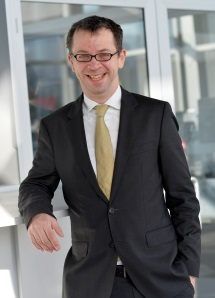
\includegraphics[scale=1]{img/BernhardHeiden.jpg} 
\vspace*{1.5cm} 
\Large
%Autor: Bernhard Andreas Heiden

%Betreuung: Univ.-Prof. Dr. Johann Götschl
%\end{Large}
\vspace{1cm}



%Selbstreferentielle Strukturen in der Entwicklung und dem Betrieb von Batch Anlagen Software Tools
%\vspace{1.5cm}


%\Large
%%Diplomarbeit
%\textbf{M A S T E R A R B E I T} \\ 
%\vspace{1cm}
%
%\large

%Untersuchung über den vierten Hauptsatz der Thermodynamik \\
%\vspace{0.5cm}
%am UNI FOR LIFE an der Geisteswissenschaftlichen Fakultät \\
%der Karl-Franzens-Universität Graz\\

\vspace{0.5cm}
%am Institut für Philosophie
%Mag. phil. Dipl.-Ing. Dr. techn. Bernhard Heiden, MBA \\
Authors: Bernhard Heiden
\Large


%\includegraphics[scale=1]{IMC.jpg}   \hspace{3cm} \includegraphics[scale=1]{UniGraz.jpg} 

\vspace{0.5cm}

Weiz, Villach, \today\ um \now
\end{center}
%\end{singlespacing}
%Einsetzen der TXC Vorlage 'Deckblatt' mäglich
\end{titlepage}

%\newpage
%\begin{center}
%\textbf{\LARGE{Ehrenwörtliche Erklärung}}
%\end{center}
%
%Ich erkläre ehrenwörtlich, dass ich die vorliegende Arbeit selbständig und ohne fremde Hilfe verfasst, andere als die angegebenen Quellen nicht benutzt, und die den Quellen wörtlich oder inhaltlich entnommenen Stellen als solche kenntlich gemacht habe. Die Arbeit wurde bisher in gleicher oder ähnlicher Form keiner anderen inländischen oder ausländischen Prüfungsbehörde vorgelegt und auch noch nicht veröffentlicht. Die vorliegende Fassung entspricht der eingereichten elektronischen Version. 




%\begin{table}
%  \caption{Eine Tabelle}
%   \begin{tabularx}{\textwidth}{XXXXXXXX} \toprule
%    Spalte1 & Spalte2 & Spalte3 & Spalte4 & Spalte5
%    & Spalte6 & Spalte7 & Spalte8 \\ \midrule
%    AA      & BB      & CC      & DD      &
%    EE      & FF      & GG      & HH      \\
%    AA      & BB      & CC      & DD
%    & EE      & FF      & GG      & HH
%    \\ \bottomrule
%  \end{tabularx}
%\end{table}

%\begin{longtable}{p{0.82\textwidth} p{0.18\textwidth}}
%%\begin{longtable}{|l|r|c|p{0.8\textwith}}|} 
%%\toprule
%Datum & Unterschrift\\
%\end{longtable}
%
%
\newpage
\addcontentsline{toc}{chapter}{Inhaltsverzeichnis}
\tableofcontents

%\onehalfspacing
%\KOMAoptions{fontsize=14pt}

%\newpage
\chapter{Teaching-Videos}
\section{Lasercutting}


\begin{enumerate}
\item
\href{https://youtu.be/sNek_bmBhno}{"Mit dem Lasercutter im Smartlab schneiden und gravieren - erste Beispiele" URL: https://youtu.be/sNek\_bmBhno}

Description: It is shown how to cut a simple geometry, a star and how to engrave a photo in the smartlab with the Epilog Laser. 

\end{enumerate}

\chapter{Project-Videos}
\chapter{Privatissimum SS18}

\section{2018\_04\_20 Privatissimum Smartlab}
\href{https://youtu.be/GYzbqOBqjh4}{"2018\_04\_20 Privatissimum Smartlab" URL:https://youtu.be/GYzbqOBqjh4}

Description: Experiment for the Triangulation with the FabsScan 100 - first live Cast in the smartlab.
\begin{itemize}
\item  Experiment for the Triangulation with the FabsScan 100  from Mr. F. Yuchen
\item Sensor news with the robot car from Mr. Y. Shi

\end{itemize} 

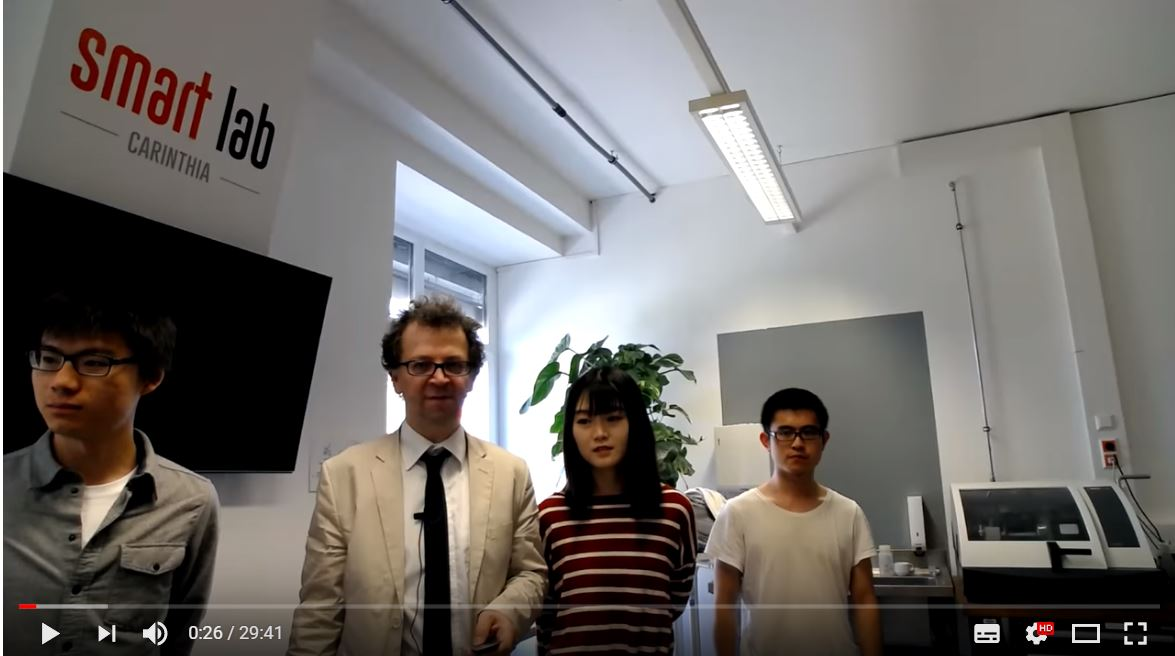
\includegraphics[scale=0.5]{img/Privatissimum1a.JPG} 

\section{2018\_04\_23 Privatissimum BII\_06}
\href{https://vc.fh-kaernten.at/pu5rme745q3n/}{2018\_04\_23 Privatissimum BII\_06 "Url: https://vc.fh-kaernten.at/pu5rme745q3n} 

and

\href{https://youtu.be/-QwOoLBjIZU}{2018\_04\_23 Privatissimum BII\_06 "Url:https://youtu.be/-QwOoLBjIZU"} 

Description: Discussion of Ukulele Project, Triangulation Experiments, RobotCar




%\chapter*{Einleitung und Motivation}

%\chapter{Der vierte Hauptsatz der Thermodynamik}







%\listoftables
%\addcontentsline{toc}{chapter}{\listtablename}
%\listoffigures


%\printbibliography[heading=bibintoc]
%\printbibliography[heading=bibnumbered]
%\printindex % Index drucken

%\printnomenclature
%

\end{document}
